\documentclass[11pt]{article}
%%%%%%%%%%%%%%%%
% Packages
%%%%%%%%%%%%%%%%

\usepackage[top=1cm,bottom=1.1cm,left=1.25cm,right= 1.25cm]{geometry}
\usepackage[parfill]{parskip}
\usepackage{graphicx, fontspec, xcolor,multicol, enumitem, setspace, amsmath, changepage}
\DeclareGraphicsRule{.tif}{png}{.png}{`convert #1 `dirname #1`/`basename #1 .tif`.png}

%%%%%%%%%%%%%%%%
% User defined colors
%%%%%%%%%%%%%%%%

% Pantone 2015 Fall colors
% http://iwork3.us/2015/02/18/pantone-2015-fall-fashion-report/
% update each semester or year

\xdefinecolor{custom_blue}{rgb}{0, 0.32, 0.48} % FROM SPRING 2016 COLOR PREVIEW
\xdefinecolor{custom_darkBlue}{rgb}{0.20, 0.20, 0.39} % Reflecting Pond  
\xdefinecolor{custom_orange}{rgb}{0.96, 0.57, 0.42} % Cadmium Orange
\xdefinecolor{custom_green}{rgb}{0, 0.47, 0.52} % Biscay Bay
\xdefinecolor{custom_red}{rgb}{0.58, 0.32, 0.32} % Marsala

\xdefinecolor{custom_lightGray}{rgb}{0.78, 0.80, 0.80} % Glacier Gray
\xdefinecolor{custom_darkGray}{rgb}{0.35, 0.39, 0.43} % Stormy Weather

%%%%%%%%%%%%%%%%
% Color text commands
%%%%%%%%%%%%%%%%

%orange
\newcommand{\orange}[1]{\textit{\textcolor{custom_orange}{#1}}}

% yellow
\newcommand{\yellow}[1]{\textit{\textcolor{yellow}{#1}}}

% blue
\newcommand{\blue}[1]{\textit{\textcolor{blue}{#1}}}

% green
\newcommand{\green}[1]{\textit{\textcolor{custom_green}{#1}}}

% red
\newcommand{\red}[1]{\textit{\textcolor{custom_red}{#1}}}

%%%%%%%%%%%%%%%%
% Coloring titles, links, etc.
%%%%%%%%%%%%%%%%

\usepackage{titlesec}
\titleformat{\section}
{\color{custom_blue}\normalfont\Large\bfseries}
{\color{custom_blue}\thesection}{1em}{}
\titleformat{\subsection}
{\color{custom_blue}\normalfont}
{\color{custom_blue}\thesubsection}{1em}{}

\newcommand{\ttl}[1]{ \textsc{{\LARGE \textbf{{\color{custom_blue} #1} } }}}

\newcommand{\tl}[1]{ \textsc{{\large \textbf{{\color{custom_blue} #1} } }}}

\usepackage[colorlinks=false,pdfborder={0 0 0},urlcolor= custom_orange,colorlinks=true,linkcolor= custom_orange, citecolor= custom_orange,backref=true]{hyperref}

%%%%%%%%%%%%%%%%
% Instructions box
%%%%%%%%%%%%%%%%

\newcommand{\inst}[1]{
\colorbox{custom_blue!20!white!50}{\parbox{\textwidth}{
	\vskip10pt
	\leftskip10pt \rightskip10pt
	#1
	\vskip10pt
}}
\vskip10pt
}

%%%%%%%%%%%
% App Ex number    %
%%%%%%%%%%%

% DON'T FORGET TO UPDATE

\newcommand{\appno}[1]
{5.2}

%%%%%%%%%%%%%%
% Turn on/off solutions       %
%%%%%%%%%%%%%%

% Off
\newcommand{\soln}[2]{$\:$\\ \vspace{#1}}{}

%%% On
%\newcommand{\soln}[2]{\textit{\textcolor{custom_red}{#2}}}{}

%%%%%%%%%%%%%%%%
% Document
%%%%%%%%%%%%%%%%

\begin{document}
\fontspec[Ligatures=TeX]{Helvetica Neue Light}

Dr. \c{C}etinkaya-Rundel \hfill Sta 101: Data Analysis and Statistical Inference \\
Duke University - Department of Statistical Science \hfill \\

\ttl{Application exercise \appno{}: \\
Inference for comparing two proportions}

\inst{$\:$ \\
Team name: \rule{10cm}{0.5pt} \\
$\:$ \\
Lab section: $\qquad$ 8:30 $\qquad$ 10:05 $\qquad$ 11:45 $\qquad$ 1:25 $\qquad$ 3:05 \\
$\:$ \\
Write your responses in the spaces provided below. WRITE LEGIBLY and SHOW ALL WORK! 
Only one submission per team is required. One team will be randomly selected and their 
responses will be discussed and graded. Concise and coherent are best!}

%%%%%%%%%%%%%%%%%%%%%%%%%%%%%%%%%%%%

\section*{On the Perils of Living Dangerously in the Slasher Horror Film}

\begin{center}

\includegraphics[width=0.5\textwidth]{figures/Scream-Ghostface}
\end{center}

The slasher horror film has been deplored based on claims that it depicts eroticized 
violence against predominately female characters as punishment for sexual activities. To test this assertion, a 
quantitative content analysis was conducted to examine the extent to which gender differences are evident in the 
association between character survival and engagement in sexual activities. Information pertaining to gender, 
engagement in sexual activities, and survival was coded for film characters from a simple random sample of 50 
English-language, North American slasher films released between 1960 and 2009.\footnote{Welsh, Andrew. 
\href{http://link.springer.com/article/10.1007/s11199-010-9762-x}{``On the perils of living dangerously in the slasher 
horror film: Gender differences in the association between sexual activity and survival."} Sex Roles 62.11-12 (2010): 762-773.}

%

Based on the data provided below, is survival for \textbf{female} characters in slasher films associated 
with sexual activity? If yes, quantify this association using a confidence interval. Make sure to check the necessary
conditions. \\

\begin{center}
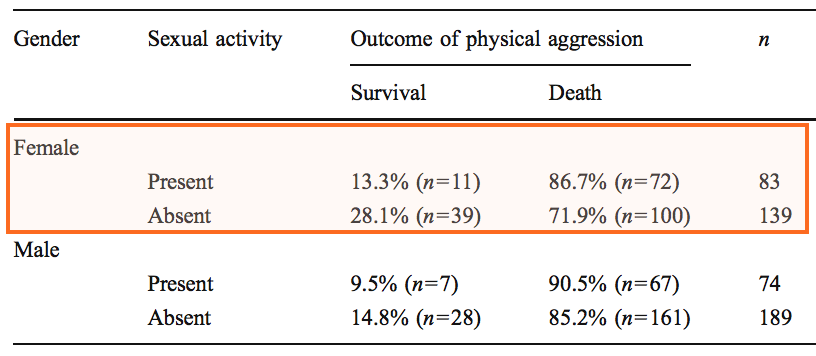
\includegraphics[width=0.6\textwidth]{figures/welsh_table3_females}
\end{center}

\pagebreak

\soln{10cm}{
Hypothesis test: \\ $\:$ \\
Conditions: \\
1. Independence: same discussion as for the males from slides \\
2. S/F: All greater than 10 \\
$\hat{p}_{pool} = \frac{11 + 39}{83 + 139} = 0.225$ \\
present: $83 * 0.225 = 18.675$ and $83 * (1 - 0.225) = 64.325$ \\
absent: $139 * 0.225 = 31.275$ and $139 * (1 - 0.225) = 107.725$ \\
Hence we can assume that the sampling distribution of the difference in two proportions is nearly normal. \\
$H_0: p_{present} = p_{absent}$ \\ 
$H_A: p_{present} \ne p_{absent}$ \\
$Z = \frac{0.133 - 0.281}{\sqrt{\frac{0.225 * (1 - 0.225)}{139} + \frac{0.225 * (1 - 0.225)}{139}}} = -2.95$ \\
$p-value = 0.0016 * 2 = 0.0032$ \\
Reject $H_0$, the data provide convincing evidence of a difference in rates of survival of female characters in
slasher movies who are and are not involved in sexual activity. \\
Confidence interval: \\ $\:$ \\
Conditions: \\
1. Independence: same as before\
2. S/F: All observed counts are greater than 10 \\
$(0.133 - 0.281) \pm 1.96 \sqrt{\frac{0.133 * (1 - 0.133)}{139} + \frac{0.281 * (1 - 0.281)}{139}}$ \\
$= -0.148 \pm 1.96 * 0.0478 =  -0.148 \pm 0.094 = (-0.242, -0.054)$ \\
We are 95\% confident that in slasher movies, 5.4\% to 24.2\% fewer female characters in who are involved in
sexual activity are expected to survive, compared to females character who are not involved in sexual activity.
}

%%%%%%%%%%%%%%%%%%%%%%%%%%%%%%%%%%%%

\end{document}